% !TeX root = ../main.tex

\chapter{相关技术简介}
本章用3个小结来对相关的技术背景做总结介绍。在第一小结中,首先对国内外的深度学习计算库进行调研分析,分析其软件架构和整体运行流程,并从中总结出其软件设计思路和架构限制。在接下来的三节中会较为详细的介绍自己参与开发的DNNCL计算库的技术背景、编程模型和运行流程。从深度学习计算库的编程模型和运行流程上分析,提出我们的核心问题,如何优化深度学习加速库的运行时过程。

\section{深度学习计算库架构分析}
深度学习计算库的主要目的是在特定的硬件环境下,针对专门的深度学习应用,结合硬件自身的特性,通过一系列优化手段,来提升深度学习算法在硬件上的表现。目前已经有很多深度学习计算库在易用性、通用性、软件设计上都表现的很优秀。例如大家所
熟知的cuDNN计算库,利用底层GPU并行处理能力强的特性,对常见的卷积神经网络算法做了很好的优化处理,并支持多深深度学习框架。

深度学习计算库可归纳为五个层次:硬件层、驱动层、运行时层(汇聚层)、编译层、框架层(应用层)。从上到下的整体架构,如图~\ref{fig:deep-learning-struct}所示。

\begin{figure}[htb]
  \centering
  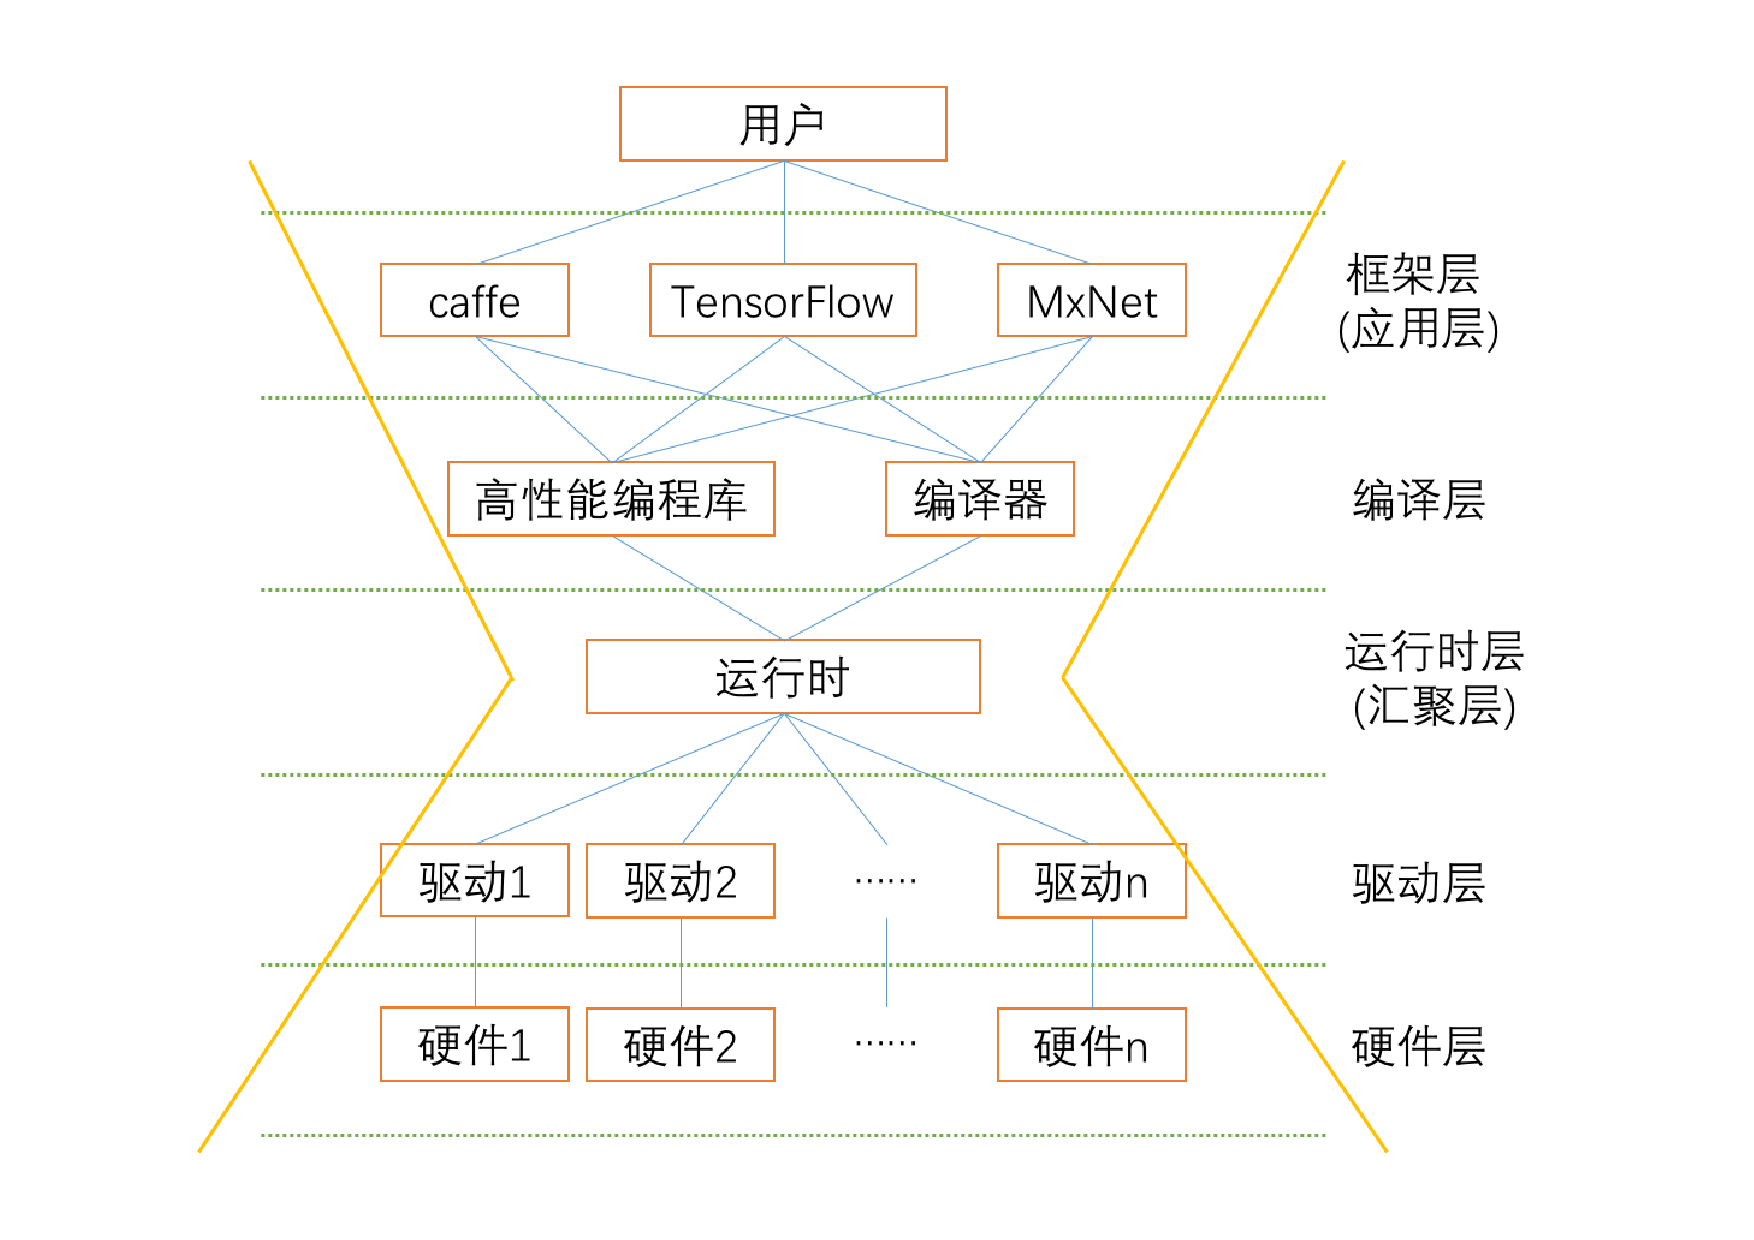
\includegraphics[width=0.6\textwidth]{deep_learning_struct.pdf}
  \caption{深度学习计算库架构图}
  \label{fig:deep-learning-struct}
\end{figure}

\subsection {硬件层}
定义:机器学习开发平台中的所有硬件设施共同构成了硬件层,包括(但不限于)主处理器(一般指CPU或通用处理器),协处理器(如基于FPGA、ASIC的加速器),存储器,输入输出设备,供电模块,以及它们的连接设备(如主板、各类桥片、总线控制器);它们共同搭建了机器学习任务开发与执行的最底层基础设施。

对上层接口:硬件层对其上层驱动层提供的信息交互接口包括(但不限于)数据接收与发送通道、控制信号接收通道、异常信号发送通道。

\subsection {驱动层}
定义:机器学习开发平台硬件层各设备所用的驱动程序称为驱动层。

功能:驱动层负责打包封装硬件层设备的基本操作,向上层运行时层提供可被调用的程序接口。基本操作包括控制数据流的输入输出(如数据拷入拷出,发送机器指令),向硬件发送控制信号(如开关设备,调整运行状态,读写寄存器),接收与处理硬件产生的异常信号(如中断处理),多任务的管理和调度等。

\subsection {运行时层(汇聚层)}
定义:运行时层是对驱动程序做进一步封装的程序,可以屏蔽底层不同硬件和驱动的差异,向上层编译层或用户提供统一的程序接口。

功能:封装上层软件不需要关心的硬件和驱动程序细节,提供机器学习任务基本操作的程序接口(如内存空间分配、数据拷贝、启动计算等),保存和加载机器学习模型及其在硬件上执行所需的机器指令等必要元素,使上层软件和用户只需要关注机器学习任务本身,而不必考虑具体硬件的差异。

\subsection {编译层}
定义:在机器学习任务中负责生成机器指令的软件称为编译层,包括编译器、针对高频算子做特殊优化的高性能编程库等\cite{randy}。

功能:接收上层框架层传入的机器学习任务的参数,编译生成硬件的二进制机器指令,传递给下层的运行时层保存下来或执行计算。

\subsection {框架层(应用层)}
定义:专注机器学习任务的算法设计,方便用户搭建自己的神经网络结构,提供便捷的训练和预测工具的软件称为框架层。

功能:接收用户设计的机器学习算法(如神经网络结构),解析出每个子任务的参数,传递给编译层生成机器指令及相关必要元素,再传递给运行时层执行计算,最终完成用户所需的机器学习任务。

可以发现整体架构呈一个沙漏形状,或称“细腰”结构,处于中间“瓶颈”环节的运行时层汇聚了上层的各类计算任务,统一了下层的所有接口,在整个机器学习开发平台的层次结构中起到了“中转站”的作用,这样设计也有利于开发的便利和保持层次的稳定,所以想要提高整体的性能,应该将重点放在提高运行时的优化上。

\section{DNNCL背景介绍}
DNNCL是DianNao系列神经网络专用处理器机器学习计算库。专用处理器顾名思义是针对某一种算法或算法家族而特殊设计的处理器, 在处理该类算法时功耗低、速度快,但是开发的成本高. 设计一个专用处理器首先需要对目标算法的特性进行详细的分析, 然后依据算法的特点来进行电路设计, 以确保最大化硬件资源利用率\cite{zhangweihua}。DianNao系列神经网络处理器从优化内存使用的角度出发而研制出来的硬件加速器, 根据机器学习算法内存分配的特点,DNNs内部设计出了不同的存储单元, 使用不同的存储单元存储不同种类数据, 最后通过流水线的方式来提高计算单元的利用率, 最终实现了以低于通用处理器约20 倍的功耗, 将计算速度提升了约117 倍, 随后使用该加速器, 设计了一个多片的DNNs 硬件系统以低于NVDIA 20M 通用图像处理器大约150 倍的功耗, 将计算速度提升了约450倍\cite{sparsenet}。

DNNCL是采用符号张量图来描述神经网络模型的结构,是一个符号式编程的库。我们知道,编程模式通常分为命令式编程(imperative style programming)和符号式编程(symbolic style programming)\cite{improgram}。命令式编程就是编写通常意义上的程序,完全按照原有逻辑执行,具有容易理解和便于调试的特点。符号式编程有用计算图来声明计算过程,编译后结合具体的输入数据执行计算。在编译阶段可以做很多的优化处理,不方便理解和调试,但能够提升内存的使用效率,加快程序运行。在现有的深度学习框架中,Torch是命令式编程的典型,完成采用命令式编程,而TensorFlow完全采用符号式编程,Caffe、MXNet则采用了两种模式混合的编程方法\cite{tensorflow}。

\begin{figure}[htb]
  \centering
  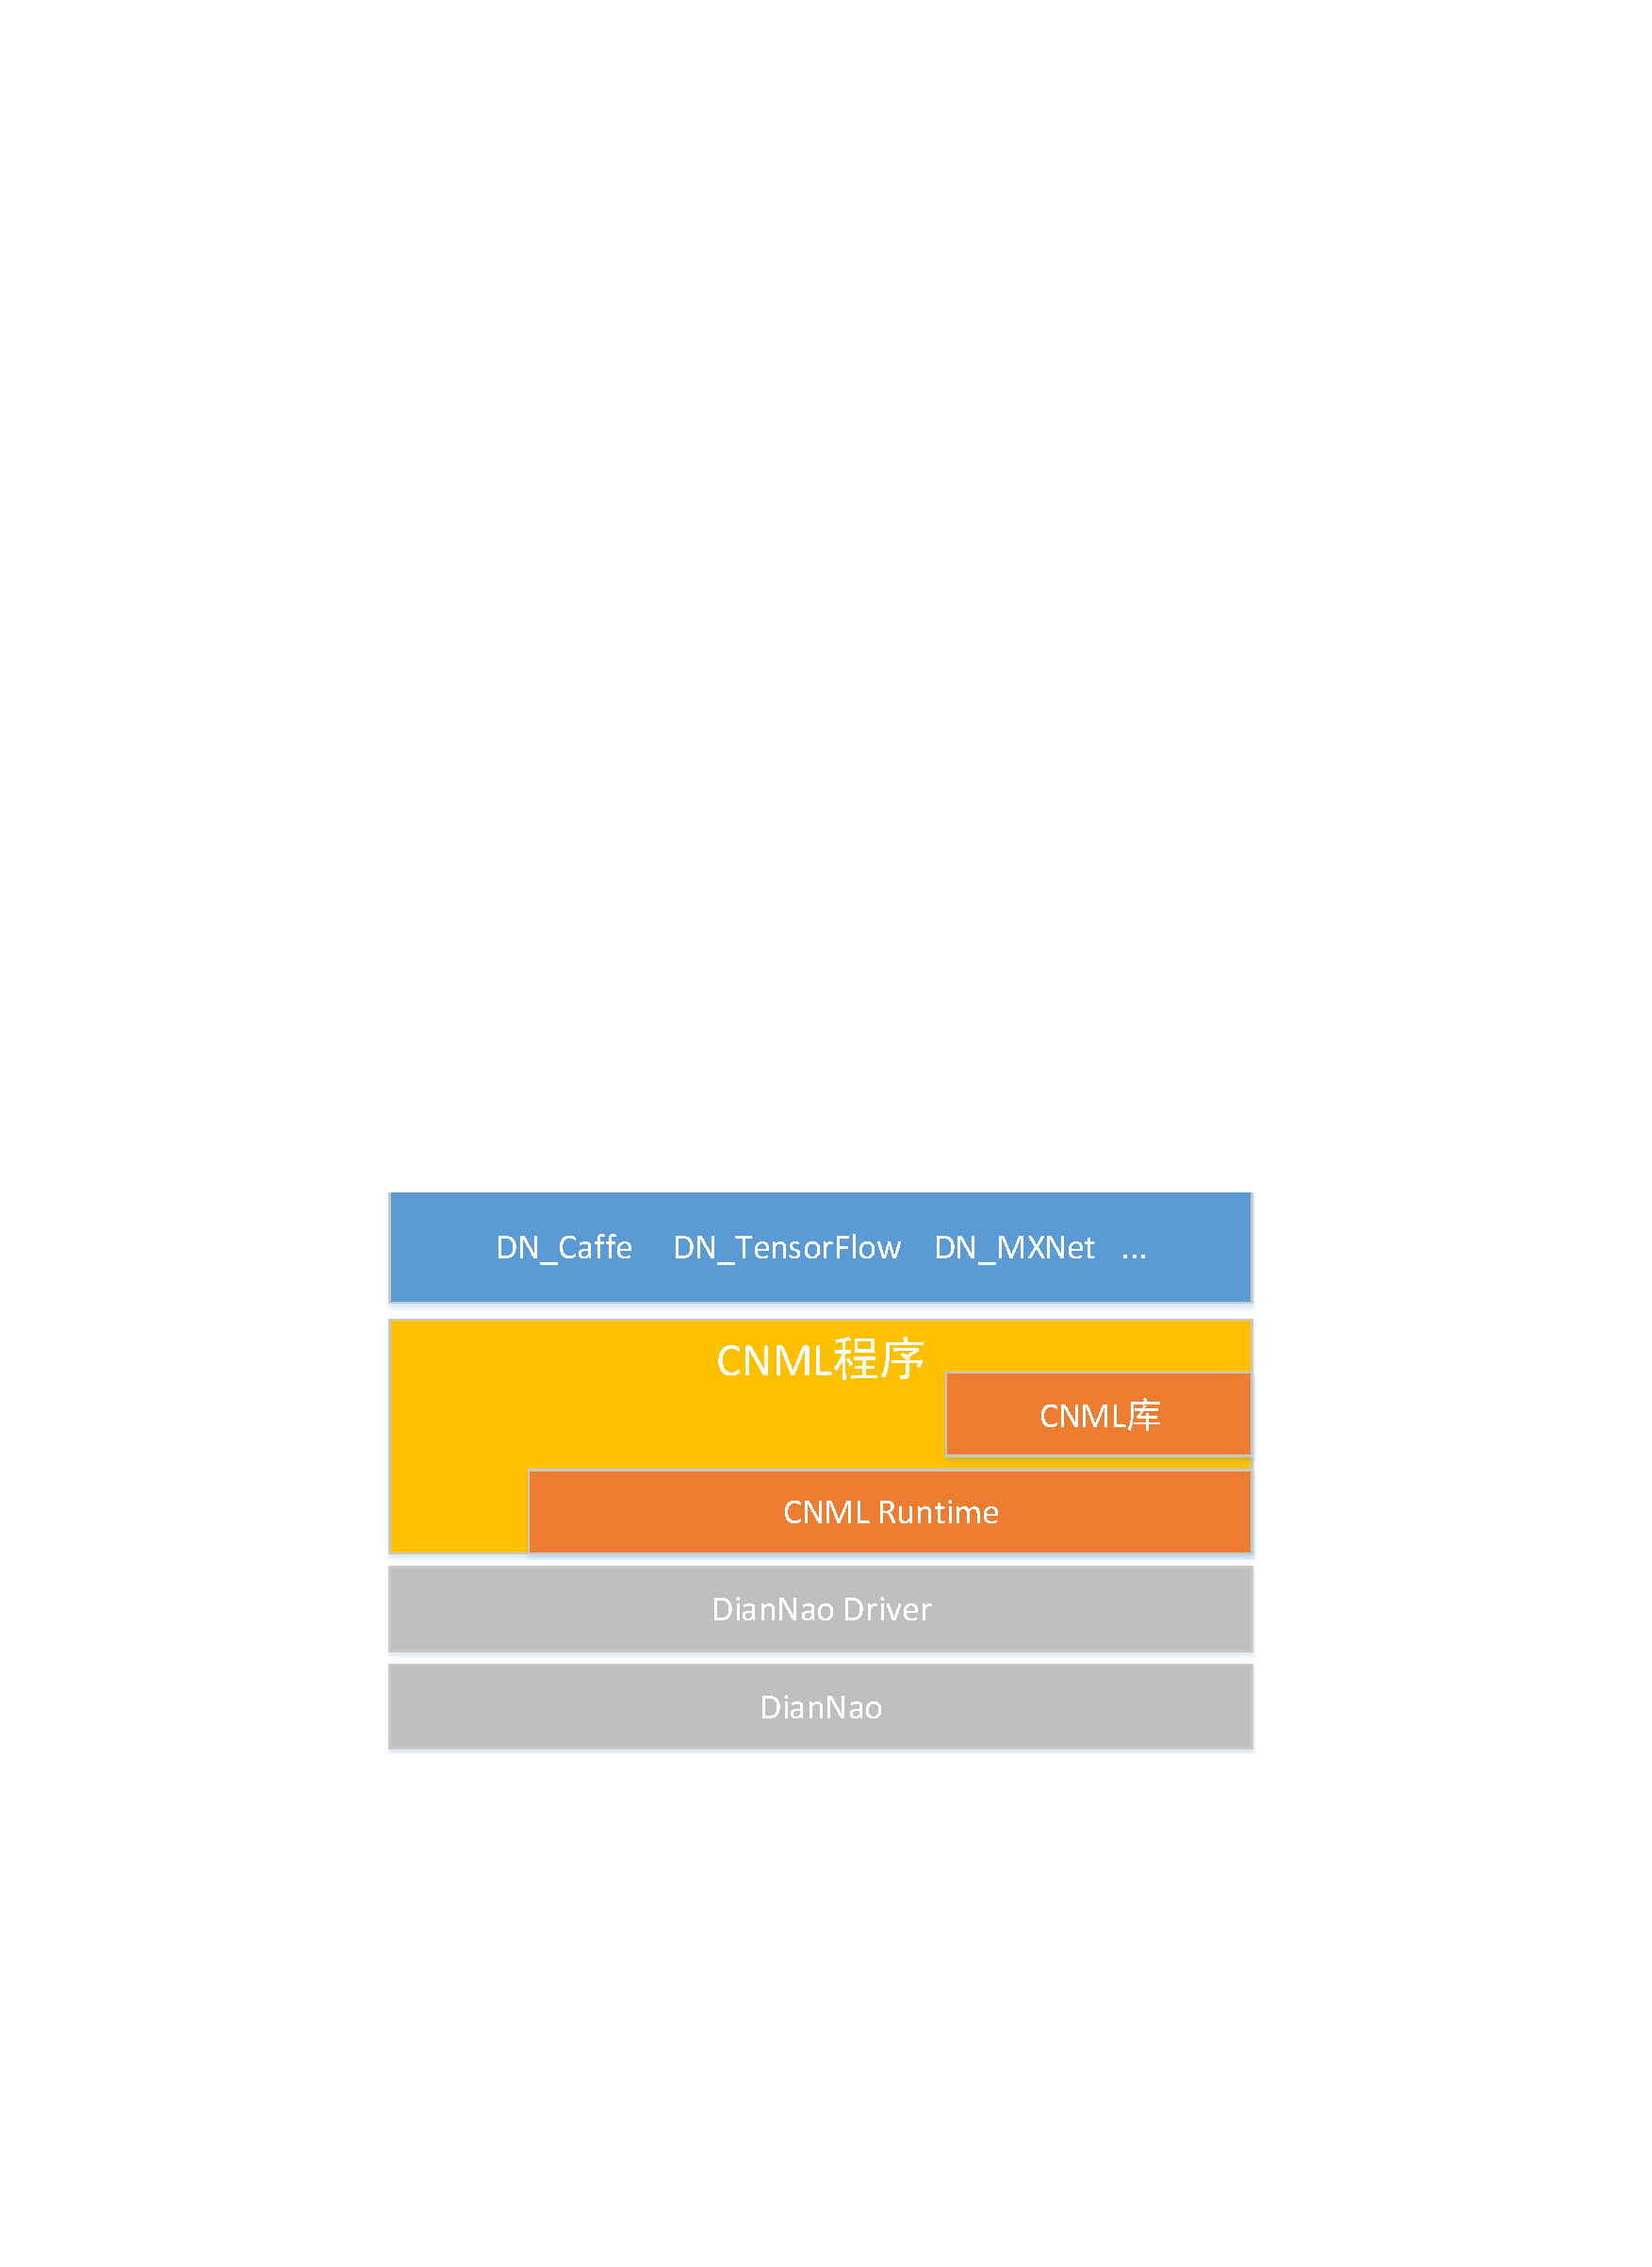
\includegraphics[width=0.4\textwidth]{dnncl_struct.pdf}
  \caption{DNNCL软件架构图}
  \label{fig:dnncl-struct}
\end{figure}

本论文所研究和实现的优化技术是基于DNNCL的,追求的目标是优化用户调用该库实现前向预测的过程。DNNCL整个架构如图~\ref{fig:dnncl-struct}所示。最底层是针对深度学习领域特点而专门研究设计的神经网路处理器;其上的驱动,直接调用各种自定义的硬件。DNNCL位于Driver之上,DNNCL的主要作用是为框架层提供各种API,其上是基于DianNao的各种深度学习框架。基于这些框架可以实现深度学习领域的各种应用,如人脸识别,自然语言处理,车牌识别等等。



\section{DNNCL编程模型介绍}
DNNCL是用数据流图做计算的,因此我们先创建一个数据流图(也称为网络结构图),如图~\ref{fig:cumputing-graph}所示,该图表示的Conv操作接收两个输入X和W做卷积计算,然后将结构传给下层的add操作,add操作接收Conv的输出和另一个输入数据B做加法运算之后再将结果传到下面的层…最终得到输出结果C。

\begin{figure}[htb]
  \centering
  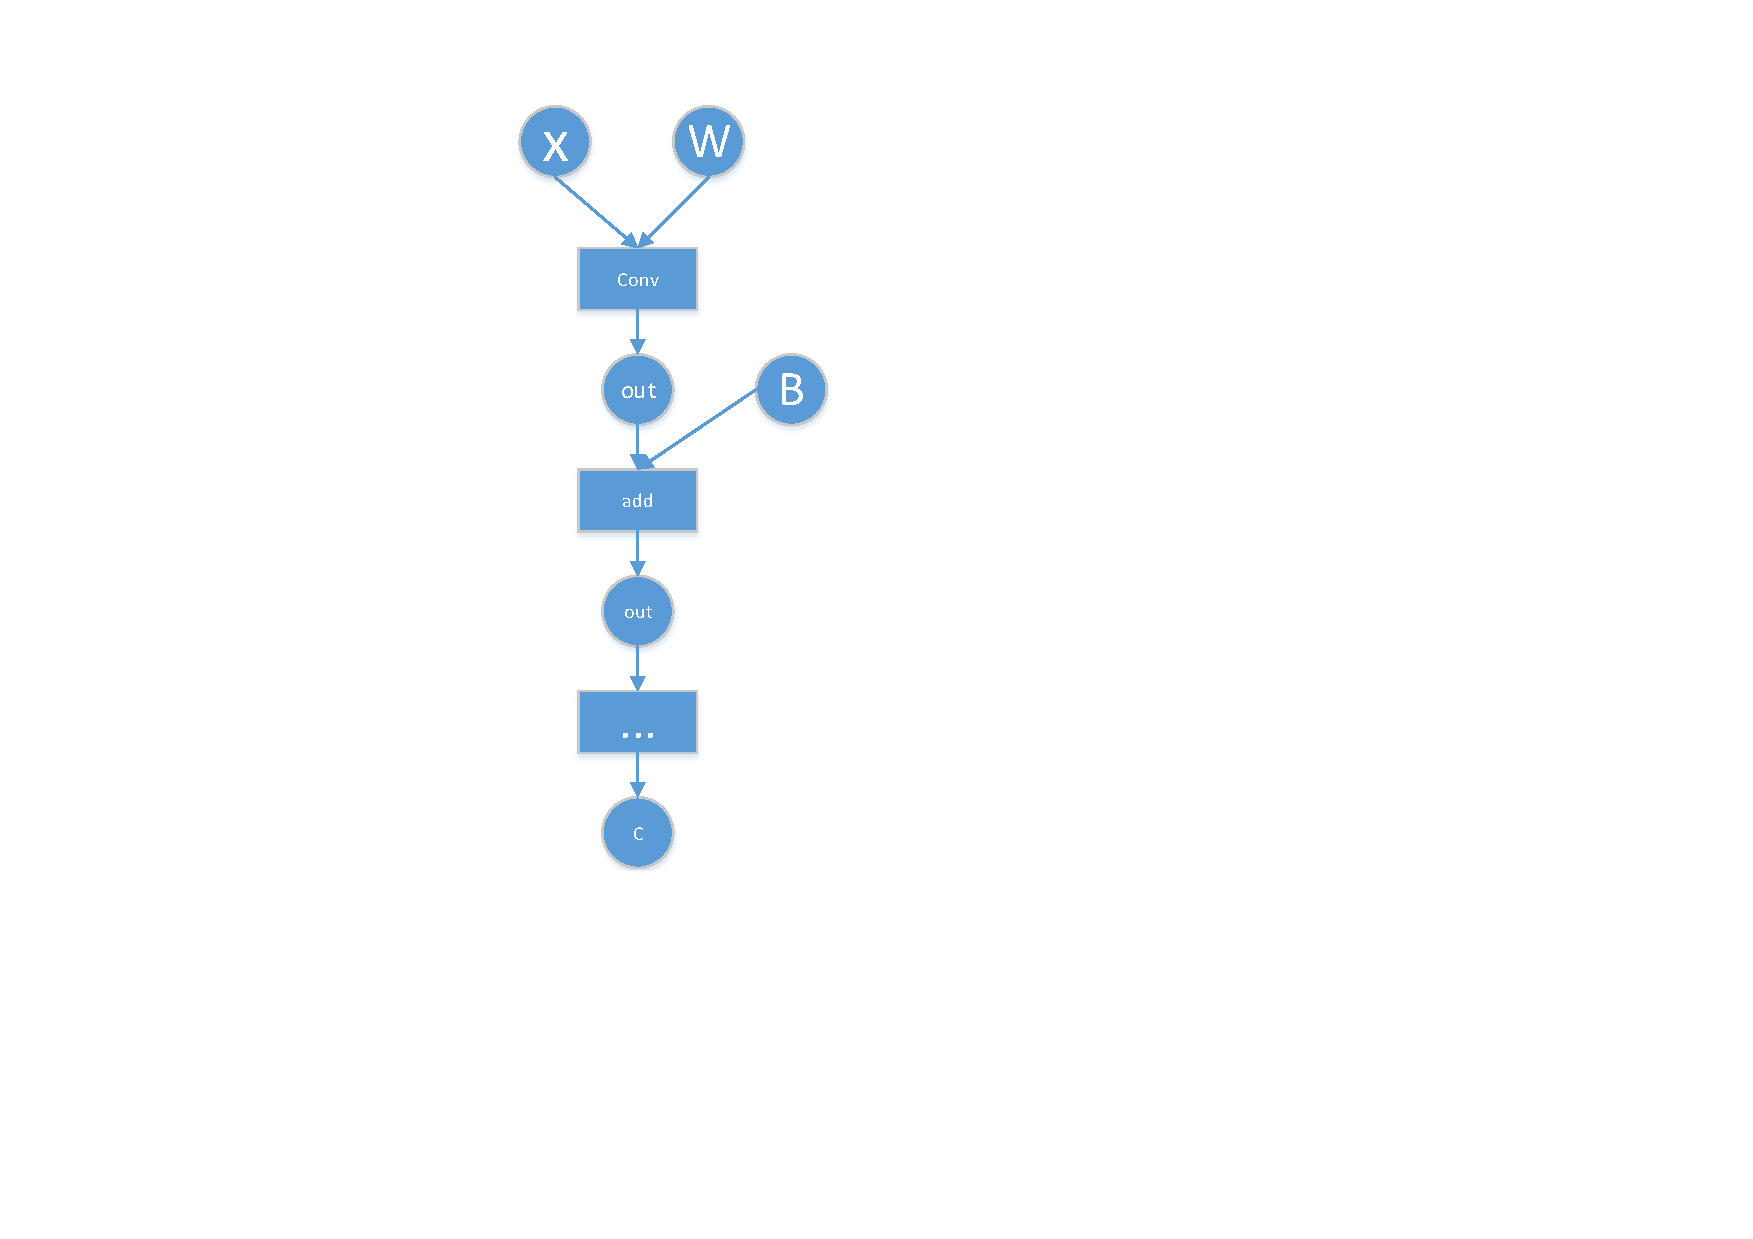
\includegraphics[scale=0.6]{computing_graph.pdf}
  \caption{计算图示例}
  \label{fig:cumputing-graph}
\end{figure}

DNNCL的数据流图是由节点(node)和边(edge)组成的有向无环图(directed acycline graph,DAG)。DNNCL由 Tensor 和 Operation 两部分组成,Tensor(张量)代表了数据流图中的边,而 Operation(操作)这个动作就代表了数据流图中节点所做的具体计算。

\subsection {边}
DNNCL的边代表数据,即张量。任意维度的数据统称为张量。在机器学习算法中,张量在数据流图中从前往后流动一遍就完成了一次前向传播(forword propagation),而残差从后向前流动一遍就完成了一次反向传播(backword propagation)。在DNNCL中,Tensor分为3类:DNNCL\_TENSOR,DNNCL\_FILTER和 DNNCL\_CONST\_TENSOR。DNNCL\_TENSOR即代表普通的输入输出;DNNCL\_FILTER即代表权值数据;DNNCL\_CONST\_TENSOR代表偏置值。DNNCL内部会根据Tensor的类型,为其分配不同的存储策略。

\subsection {节点}
图中的节点又称为算子,它代表一个操作(operation,OP),一般用来表示施加的数学运算,表~\ref{tab:compute-node}列举了一些DNNCL实现的算子。算子支持表所示的张量的各种数据属性,并且需要在建立图的时候确定下来。

\begin{table}[htb]
  \centering\small
  \caption{常见运算节点举例}
  \label{tab:compute-node}
  \begin{tabular}{ll}
    \toprule
    节点类别   &  示例                                     \\
    \midrule
    数学运算操作 & Add、Subtract、Multiply、Div、Exp、Log、Greater、Less... \\
    数组运算操作 & Concat、Split、Slice、Shape、Rank... \\
    矩阵运算操作 & MatMul、Transpose...     \\
    神经网络构建操作 & SoftMax、Convolution2D、Relu、Sigmoid、pool... \\
    \bottomrule
  \end{tabular}
\end{table}

\subsection {图}
把操作任务描述成有向无环图。DNNCL构建图的方法分为三步,第一步是创建边;第二步,将边作为创建节点的输入输出参数来创建节点;第三步通过接口将节点连接在一起构成图。

\subsection {队列}
启动图的第一步是创建一个队列(queue)对象。队列提供在图中执行操作的一些方法。一般的模式是,建立队列,此时会生成一个计算任务的队列,在队列中添加计算图,然后执行。在调用前向计算接口来执行图时,需要填充一些输入Tensor;取回的结果类型根据输入的类型而定。

\subsection {设备}
设备(device)是指执行计算任务的硬件,拥有自己的地址空间并可以执行计算任务,DNNCL为了实现分布式执行操作,充分利用计算资源,可以明确指定当前的操作在哪个设备上执行。

\subsection {内核}
操作(operation)是对抽象操作(如 matmul 或者 add)的一个统称,而内核(kernel)则是能够运行在特定设备(如 CPU、GPU)上的一种对操作的实现。因此,同一个操作可能会对应多个内核\cite{dongmian}。当自定义一个操作时,需要把新操作和内核通过注册的方式添加到系统中。

\section{DNNCL运行流程}
DNNCL是个声明式编程库,运行流程如图~\ref{fig:dnncl-run-process}所示。

\begin{figure}[htb]
  \centering
  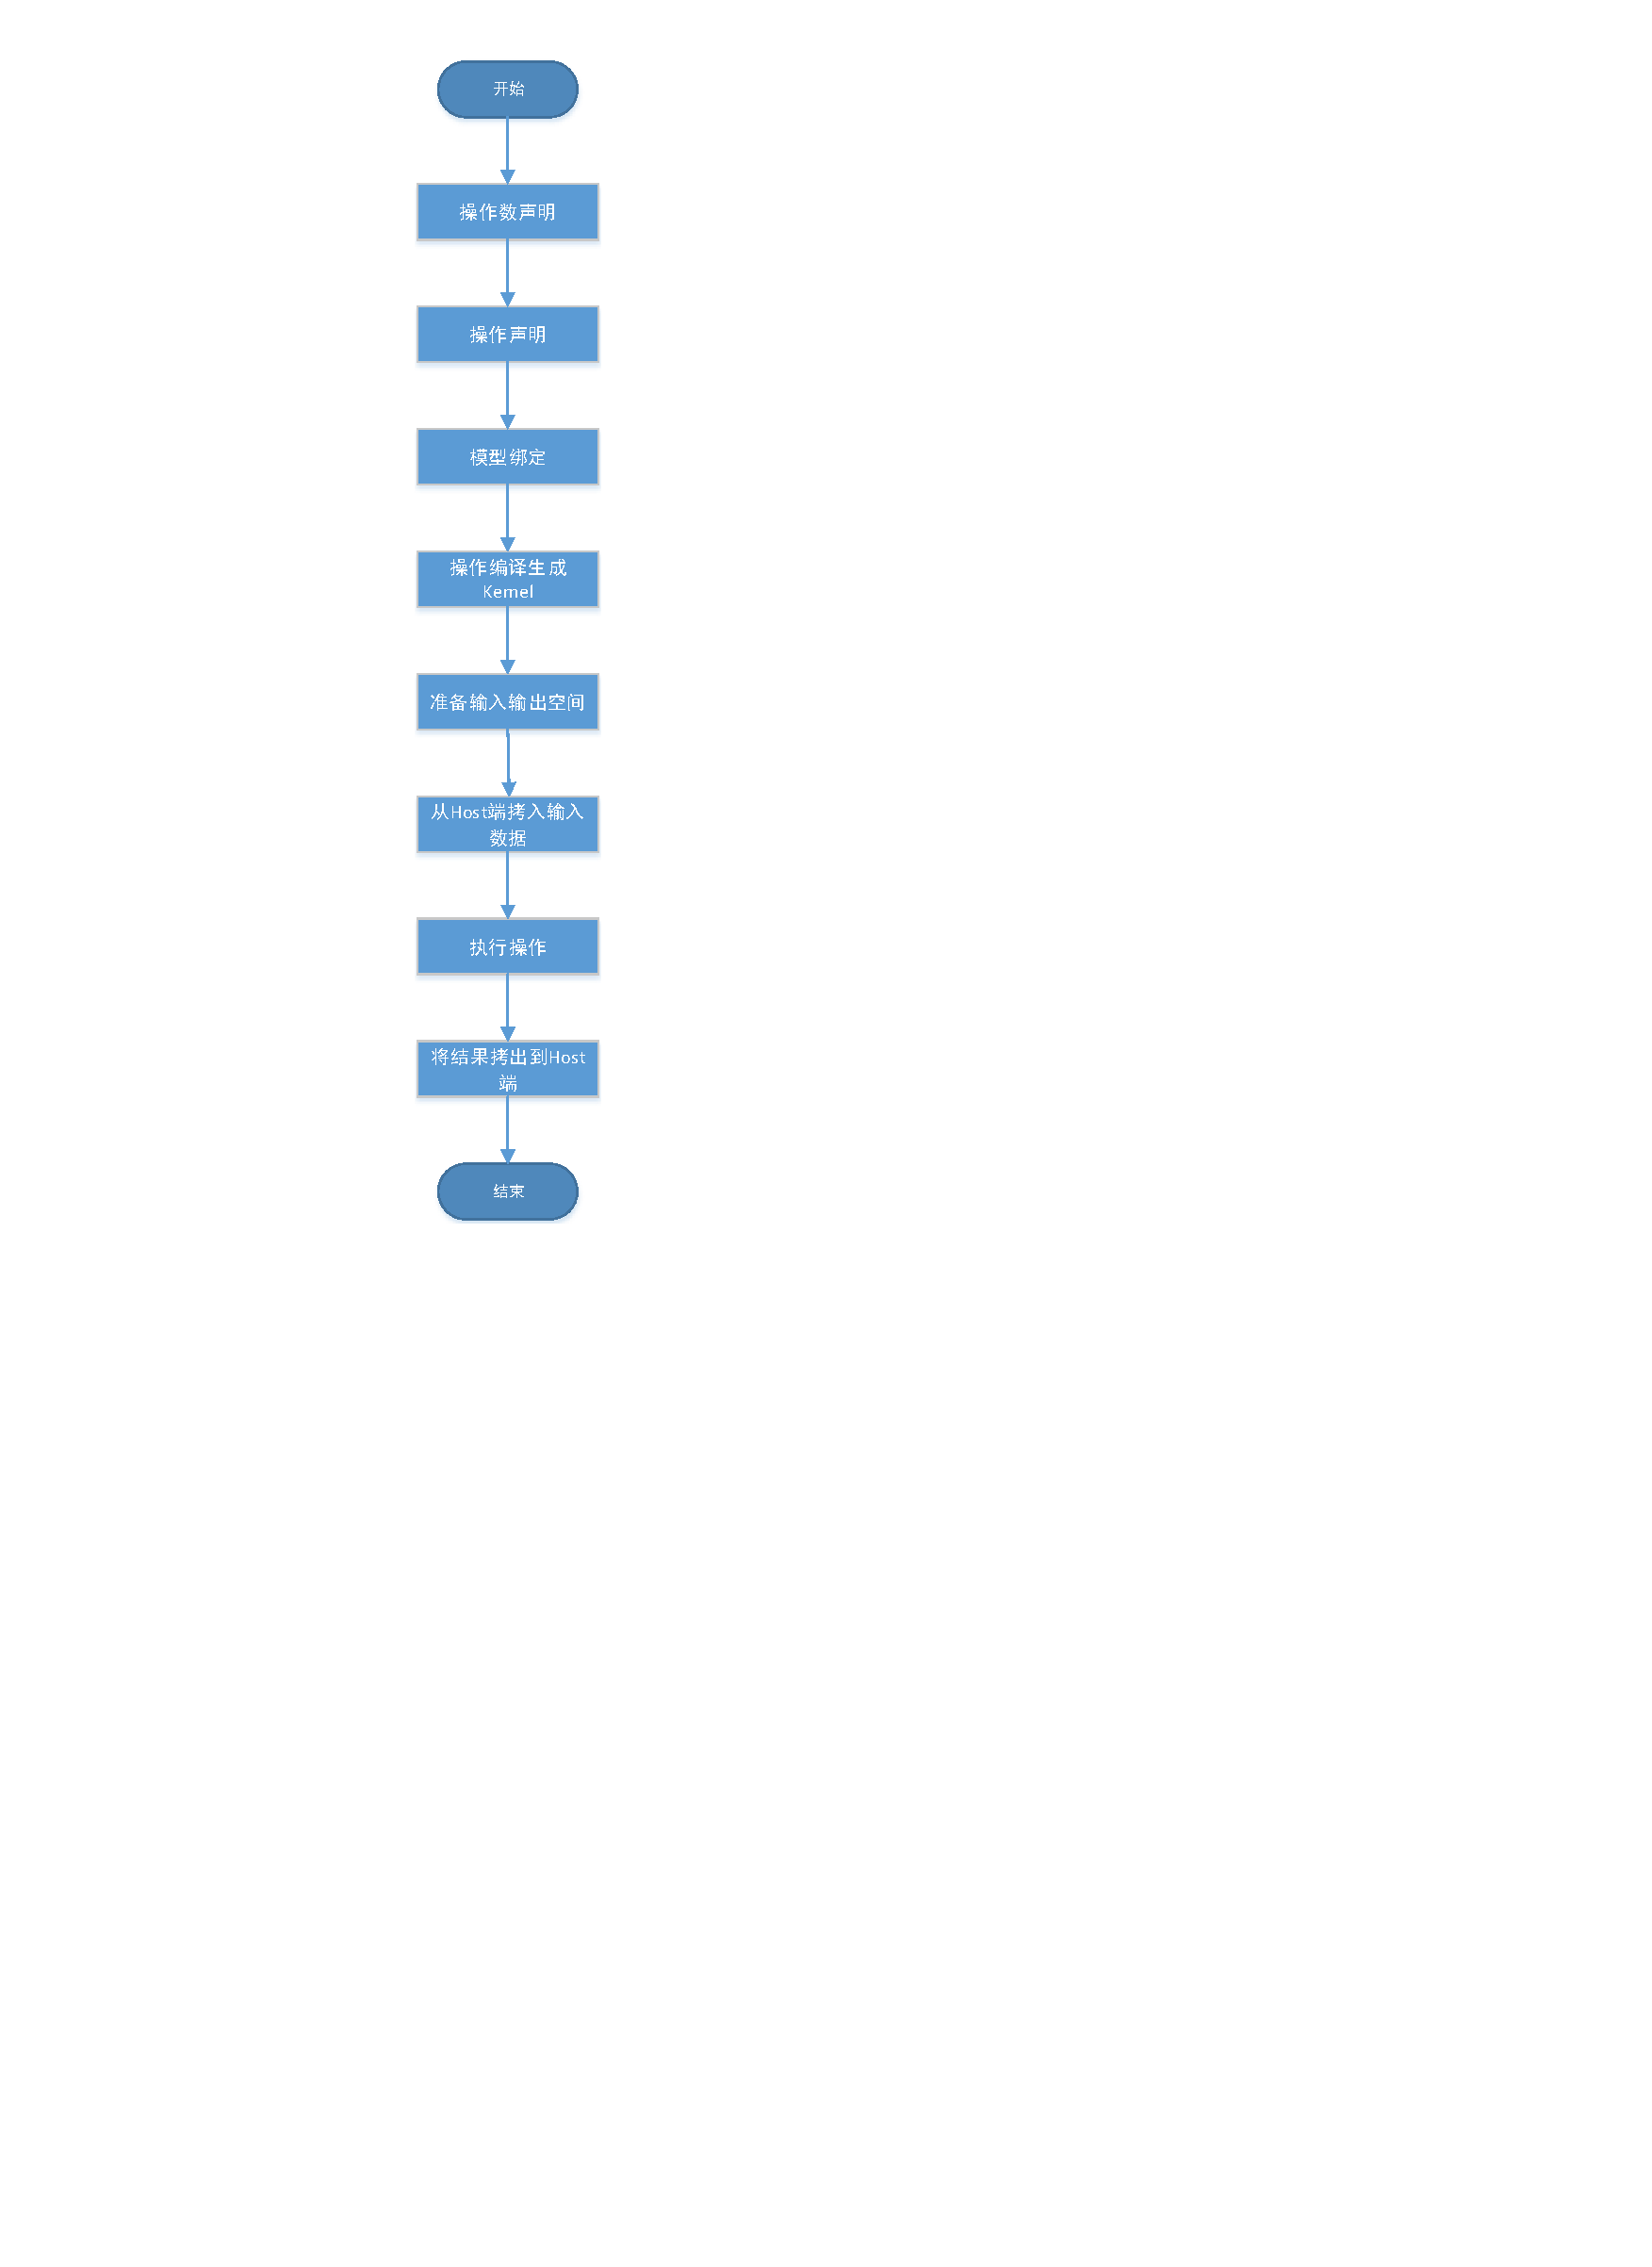
\includegraphics[width=0.15\textwidth]{dnncl_run_process.pdf}
  \caption{DNNCL运行流程图}
  \label{fig:dnncl-run-process}
\end{figure}

对于单个操作的运算,主要分为以下几步:操作数声明、操作声明、模型绑定、操作编译、Host 端准备输入输出空间并为该输入空间赋予相应的值、Device 端准备输入输出空间,拷贝 Host 端的输入数据到 Device 端,操作具体执行,拷贝 Device 端的输出数据到 Host 端。

操作数声明:即创建Tensor,设置Tensor属性,包括Tensor类型,数据维度、数据类型、数据摆放顺序等信息。数据摆放顺序指的是host端的图片数据在内存中是按哪种顺序摆放的,例如NCHW和NHWC等,N代表图片的数量,C代表图片的通道,H代表图片的高,W代表图片的宽。操作声明:即创建Operation,Op的输入包括创建的Tensor和计算所需的一些额外参数信息。

模型绑定:即构建计算图的过程,将单Op连接到一个构成一个复杂的融合Op。一个复杂的神经网路就是一个或者多个融合Op。

操作编译:即根据具体的硬件平台将操作编译生成能在设备上运行的Kernel的过程。在编译过程中能做些优化措施,例如图优化,数据量化等。在该阶段的优化是透明的,对用户不可见。

准备输入输出空间:即host端和device端准备输入输出数据的空间。在神经网络的推理过程中,只有神经网络的输入数据是动态变化的,其余参与计算的静态数据(filter和bias)是保持不变的。在编译过程中,静态数据会被提前保存到kernel中,所以在实际计算的过程中,只需要为输入数据动态分配空间。

从Host端拷入输入数据到Device端:即将Host端的输入数据拷贝到Device端的过程。由于DNNCL的设备端只支持以一种特定的数据摆放顺序进行计算,但是Host端数据顺序可能有多种,所以在拷贝数据的过程中还涉及到转数的过程。即将host端的数据按照Device端的顺序重新排布。

执行操作:即启动设备,执行具体计算的过程。

拷贝Device端计算结果到Host端:即将Device端的计算结果拷贝到Host端的过程,和拷贝输入数据一样,该过程也涉及到转数的过程。

\section {本章小结}
本章详细介绍了本文实验平台的基础知识,包括DNNCL的设计理念、编程模型和运行流程。DNNCL库是声明式编程,将计算图定义和图计算完成分开,便于优化神经网络的计算过程来提升计算速度。编程模型中简要介绍了库中的边、节点、图、设备、会话、内核等核心概念,简要说明了如何去构建计算图。在运行流程一节中简要介绍了用户在DNNCL上完成神经网络计算所进行的主要步骤,包括声明操作数、声明操作、模型绑定、编译操作、拷贝 Host 端的输入数据到 Device 端、执行具体操作,拷贝 Device 端的输出数据到 Host 端等过程。
